\subsection{Bayesian Linear Regression}\label{ssec:regression}

\begin{figure*}[t]
    \centering
    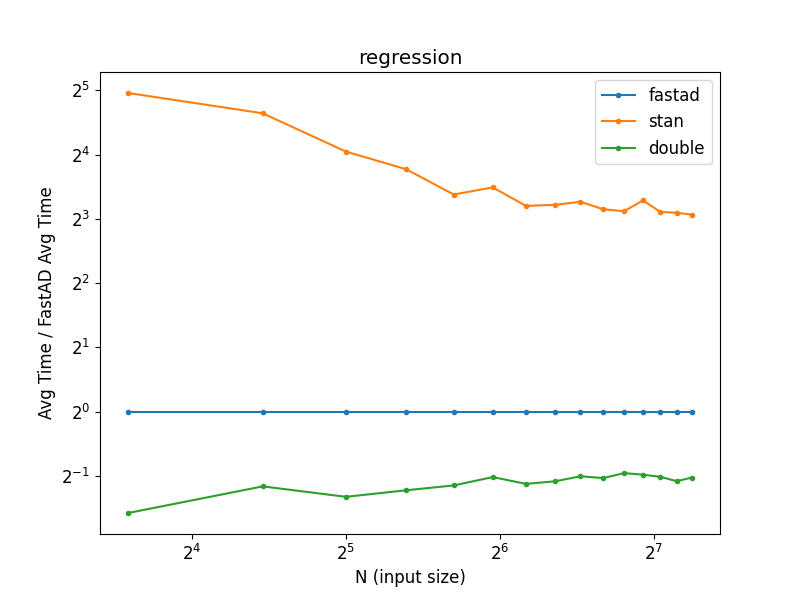
\includegraphics[width=\textwidth]{figs/regression_fig.png}
    \caption{%
        Bayesian linear regression benchmark of Stan against FastAD 
        plotted relative to FastAD average time.
    }\label{fig:regression}
\end{figure*}

This section marks the first macro-benchmark example.
We consider the following Bayesian linear regression model:
\begin{align*}
    y &\sim N\paren{X\cdot w + b, \sigma^2} \\
    w &\sim N\paren{0,1} \\
    b &\sim N\paren{0,1} \\
    \sigma &\sim Unif\paren{0.1, 10.}
\end{align*}
The target function is the log of the joint probability density function (up to a constant).
For this benchmark, we only consider Stan since they specialize in differentiating such functions
and because the other libraries were not well-suited to implement this efficiently.
The fill function for this functor will resize a vector of size $N = 2^K$ as $\tilde{N} = (K + 1) \cdot 10 + 2$,
where the first $(K+1) \cdot 10$ values refer to $w$ and the rest refer to $b$ and $\sigma$, respectively.
It also resizes its private members for $y \in \R^{1000}$ and $X \in \R^{1000 \times \tilde{N}}$.
Here, $y$ and $X$ are constants.
All quantities are randomly generated uniformly in $(-1,1)$ range,
but $\sigma$ is replaced with its absolute value plus $0.1$ to make it strictly positive.

The following is the functor overload for Stan:
\begin{lstlisting}[style=customcpp]
    using vec_t = Eigen::Matrix<var, Eigen::Dynamic, 1>;
    size_t N = (x.size() - 2);
    Eigen::Map<const vec_t> w(x.data(), N);
    auto& b = x(N);
    auto& sigma = x(N + 1);
    return normal_lpdf(y, multiply(X, w) + b * vec_t::Ones(1000), sigma) +
            normal_lpdf(w, 0., 1.) +
            normal_lpdf(b, 0., 1.) -
            uniform_lpdf(sigma, 0.1, 10.);
\end{lstlisting}
Note that we tried removing \verb|vec_t::Ones(1000)|, but the program failed to compile.
The following is the functor overload for FastAD, which is quite similar:
\begin{lstlisting}[style=customcpp]
    size_t N = (x.size() - 2);
    ad::VarView<T, ad::vec> w(x.data(), x.data_adj(), N);
    ad::VarView<T> b(x.data() + N, x.data_adj() + N);
    ad::VarView<T> sigma(x.data() + N + 1, x.data_adj() + N + 1);
    return ad::normal_adj_log_pdf(y, ad::dot(X, w) + b, sigma) 
            + ad::normal_adj_log_pdf(w, 0., 1.)
            + ad::normal_adj_log_pdf(b, 0., 1.)
            + ad::uniform_adj_log_pdf(sigma, 0.1, 10.);
\end{lstlisting}
Fig.\ref{fig:regression} shows the benchmark results.

FastAD outperforms Stan by 8 times for the largest $N$.
The trend stabilizes starting from around $N=70$.
It is interesting to see that FastAD is only 2 times slower than the \verb|double| baseline,
despite the model consisting of a large matrix multiplication and many normal log-pdf functions.
This is because the compiler was able to optimize-out backward-evaluation for $X$.
FastAD creates a wrapper class for constants and implements a no-op for backward-evaluation.
If we assume that the most expensive operation is the matrix multiplication,
AD evaluation approximately takes 2 matrix multiplication with a matrix and a vector.
With that in mind, if we approximate the manually-written gradient computation
to be two times the baseline, which is a lower bound, the relative time of FastAD to this approximation is
$1.018$, i.e.\ less than $ 1.8\%$ overhead from the manually-written code.
